\documentclass{book}

\usepackage{amssymb}
\usepackage{amsmath}
\usepackage{amsthm}
\usepackage{arydshln}
\usepackage{calc}
\usepackage{cancel}
\usepackage{caption}
\usepackage{cite}
\usepackage{color}
\usepackage{enumitem}
\usepackage{esint}
\usepackage{etoolbox}
\usepackage{float}
\usepackage{framed}
\usepackage{fullpage}
\usepackage{gensymb}
\usepackage[margin=1in]{geometry}
\usepackage{graphicx}
\usepackage{listings}
\usepackage{multirow}
\usepackage{subfiles}
\usepackage{rsfso}
\usepackage{tikz}
\usepackage{tikz-3dplot}
\usepackage{ushort}
\usepackage{wrapfig}
\usepackage{xcolor}
\usepackage{soul}
\usepackage{epstopdf}

% pdf versions
\pdfoptionpdfminorversion=7

% handle page stretching
\raggedbottom

% Graphics file location
\graphicspath{{Graphics/}{../Graphics/}}

% Use for drawings
\usetikzlibrary{angles,arrows,calc,decorations,intersections,patterns,positioning,quotes,shapes}
\usetikzlibrary{shapes.geometric}
\usetikzlibrary{decorations.pathreplacing}
\newcommand{\midarrow}{\tikz \draw[-latex] (0,0) -- +(.1,0);}

% Tikz commands for drawing block diagrams, etc...
\tikzset{%
	block/.style    = {draw, rectangle, minimum height = 2em, minimum width = 2em},
	sum/.style      = {draw, circle}, % Adder
	input/.style    = {fill=white, rectangle}, % Input
	output/.style   = {fill=white, rectangle}, % Output
	waypoint/.style   = {coordinate}, % Output
}

\tikzset{%
	startstop/.style= {draw, rectangle, rounded corners, minimum width=2cm, minimum height=1cm,text centered},
	inout/.style    = {draw, trapezium, trapezium left angle=70, trapezium right angle=110, minimum width=2cm, minimum height=1cm, text centered},
	process/.style  = {draw, rectangle, minimum width=2cm, minimum height=1cm, text centered},
	decision/.style = {draw, diamond, minimum width=1.5cm, minimum height=1cm, text centered, diamond, aspect=2},
	arrow/.style    = {thick,-latex,>=stealth},		
}

\tikzset{
	saveuse path/.code 2 args={
		\pgfkeysalso{#1/.style={insert path={#2}}}%
		\global\expandafter\let\csname pgfk@\pgfkeyscurrentpath/.@cmd\expandafter\endcsname
		% not optimal as it is now global through out the document
		\csname pgfk@\pgfkeyscurrentpath/.@cmd\endcsname
		\pgfkeysalso{#1}},
	/pgf/math set seed/.code=\pgfmathsetseed{#1}}

% Define Laplace, Fourier transform symbols
\newcommand{\LT}{\mathcal{L}}
\newcommand{\FT}{\mathcal{F}}

% Define adjugate function
\newcommand{\adj}{\text{adj}}

% Define rank function
\newcommand{\rank}{\text{rank}}

% commands to speed up writing j\omega and s-plane
\newcommand{\jw}{j\omega}
\newcommand{\spl}{s\textrm{-plane}}
\newcommand{\wt}{\omega t}
\newcommand{\Lm}{\textrm{Lm }}
% Clean up overline/underline for math mode
\def\obar#1{\bar{#1}}
\def\ubar#1{\ushort{#1}}

\newcommand{\exmp}{\subsubsection*{Example}}
\newcommand{\nib}{\noindent$ \bullet\ $}


\begin{document}
\chapter*{Lecture 15}
Last lecture:\\
\textbf{Bode Plots}
\begin{itemize}
	\item Superposition
	\begin{itemize}
		\item $ \Lm M_{total} = \sum\Lm M_{components} $
		\item $  \phi_{total} = \sum \phi_{components} $
	\end{itemize}
	\item Poles/zeros have an effect for $ \omega>pole/zero $
	\item Zeros add $ 90^\circ $ of phase and add 20dB/decade of slope to $ \Lm M$
	\item Poles subtract $ 90^\circ $ of phase and subtract 20dB/decade of slope to $ \Lm M$
\end{itemize}
\textbf{Feedback}
\begin{center}
	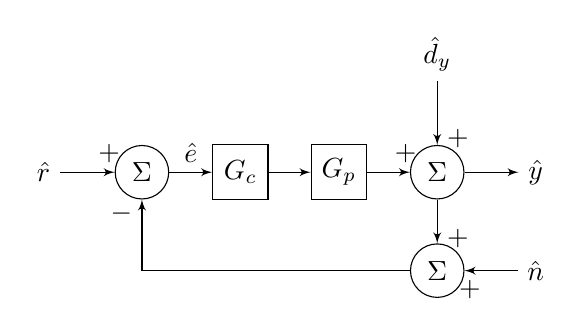
\begin{tikzpicture}[node distance=1.25cm,auto,>=latex']
	\node [input] (r) {$\hat{r}$};
	\node [sum] (sumr) [right of=r] {$\Sigma$};
	\node [block] (gc) [right of=sumr] {$ G_c $};
	\node [block] (gp) [right of=gc] {$ G_p $};
	\node [sum] (sumy) [right of=gp] {$\Sigma$};
	\node [output] (y) [right of=sumy]{$\hat{y}$};
	\node [sum] (sumn) [below of=sumy] {$\Sigma$};
	\node [input] (n) [right of=sumn,align=center]{$ \hat{n} $};
	\node [input] (dy) [above of=sumy,node distance=1.5cm]{$ \hat{d}_y $};
	
	\draw[->] (r) -- node[pos=0.9] {$+$} (sumr);
	\draw[->] (sumr) -- node {$\hat{e}$} (gc);
	\draw[->] (gc) -- (gp);
	\draw[->] (gp) -- node[pos=0.9] {$+$} (sumy);		
	\draw[->] (dy) -- node[pos=0.9] {$+$} (sumy);
	\draw[->] (sumy) -- (y);
	\draw[->] (sumy) -- node[pos=0.9] {$+$} (sumn);
	\draw[->] (n) -- node[pos=0.9] {$+$} (sumn);
	\draw[->] (sumn) -| node[pos=0.9] {$-$} (sumr);
	\end{tikzpicture}
\end{center}
\begin{itemize}
	\item The closed-loop system will be good at dealing with noise ($ \hat{n} $) and disturbances ($ \hat{d}_y $) if the $ \Lm M $ plot of $ G_cG_p $ (the open-loop transfer function) has a good shape:
		\begin{center}
			\begin{tikzpicture}[scale=1]
				\draw (0,3.5) node[left] {$\Lm M$} |- (5,0) node[below left] {$ \omega $};
				
				\draw[dashed] (0,1.5) node[left] {0dB} -| (2.5,0) node[below] {$ \omega_c $};
				\draw[thick] (0,3)-- (0.78125,2.375) ..controls (1.5625,1.75) .. (2.5,1.5) ..controls (3.4375,1.25) .. (4.21875,.625) -- (5,0);
				\node at (0.78125,2.375) {\begin{tikzpicture}[scale=0.5] \draw[dashed,rotate=-40] (0,0) ellipse (2.5 and 0.5); \end{tikzpicture}};
				\node at (2.5,1.5) {\begin{tikzpicture}[scale=0.5] \draw[dashed,rotate=-15] (0,0) ellipse (2 and 0.5);\end{tikzpicture}};
				\node at (4.21875,.625) {\begin{tikzpicture}[scale=0.5] \draw[dashed,rotate=-40] (0,0) ellipse (2.5 and 0.5); \end{tikzpicture}};
				
				\draw[-latex] (1.5,3.25) node[right,align=left] {Good disturbance\\rejection.} -- (1,2.5625);
				\draw[-latex] (3,2.375) node[right,align=left] {Good stability margins.} -- (2.6875,1.6875);
				\draw[-latex] (4.375,1.5) node[right,align=left] {Good noise\\attenuation.} -- (4.1875,1);
			\end{tikzpicture}
		\end{center}	
	\item Designing $ G_c $ to give the Bode plot of $ G_cG_p $ a good shape is call ``loop-shaping''.
\end{itemize}	
\textbf{Internal Stability}
\begin{itemize}
	\item Roots of $ 1+G_cG_p $ strictly in LHP
	\item All hidden poles are strictly in LHP ($ G_c $ does not cancel unstable RHP poles in $ G_p $)
\end{itemize}

\noindent This lecture:
\begin{itemize}
	\item Closed-loop stability and robustness
	\item Transient performance
\end{itemize}

\section*{Closed-Loop Stability}
How can we tell if a closed-loop feedback system is stable by looking at the loop gain?
\begin{center}
	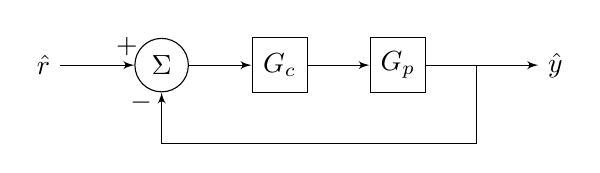
\begin{tikzpicture}[node distance=1.50cm,auto,>=latex']
	\node [input] (r) {$\hat{r}$};
	\node [sum] (sumr) [right of=r] {$\Sigma$};
	\node [block] (gc) [right of=sumr] {$ G_c $};
	\node [block] (gp) [right of=gc] {$ G_p $};
	\node [output] (y) [right of=gp,node distance=2cm]{$\hat{y}$};
	\node [waypoint] (wp) [below of=gp,node distance=1cm] {};
	
	\draw[->] (r) -- node[pos=0.9] {$+$} (sumr);
	\draw[->] (sumr) -- (gc);
	\draw[->] (gc) --  (gp);
	\draw[->] (gp) -- (y);
	\draw[->] ($ (gp)!0.5!(y) $) |- (wp)-| node[pos=0.9] {$-$} (sumr);
	\end{tikzpicture}
\end{center}
\[ T = \frac{G_cG_p}{1+G_cG_p} \]
\begin{itemize}
	\item If $ s_1 $ is a closed-loop pole then $ 1+G_c(s_1)G_p(s_1)=0 $.
	\item If the closed-loop system is stable, then $ s_1 = a+j\omega_1 $ has $ a<0 $.
	\item At the stability limit, $ s=j\omega_1 $ for at least one closed-loop pole.
	\item $ 1+G_c(s_1)G_p(s_1)=0 \quad\Rightarrow\quad 1+G_c(j\omega_1)G_p(j\omega_1)=0 $
	\item We have already been plotting $ \Lm $ and $ \phi $ of $ G_c(\jw)G_p(\jw) $. So, $ \omega_1 $ will be a particular $ \omega $ on our Bode plots.
	\item Let's look at this equation in terms of $ \Lm $ and $ \phi $:
	\[ 1+G_c(\jw_1)G_p(\jw_1)=0 \quad\Rightarrow\quad G_c(\jw_1)G_p(\jw_1)=-1 \]
	\[ \Lm M(\omega_1) = \Lm G_c(\jw_1)G_p(\jw_1) = \Lm(1) = 0dB \]
	\[ \phi(\omega_1) = \arg G_c(\jw_1)G_p(\jw_1) = \arg (-1) = \tan^{-1}\left(\frac{0}{-1}\right) = -180^\circ \]
	\item Our system is marginally stable (which is BIBO unstable):
	\begin{center}
		\begin{tikzpicture}[xscale=1.25]
			\draw (0,3.5) node[left] {$\Lm M$} |- (4,0) node[below left] {$ \omega $};
			\draw (0,3.25) -- (0.5,3) ..controls (2,2.25) .. (2.5,1.25) -- (3.125,0);
			\draw[dashed] (0,2.125) node[left]{0dB} -- (2,2.125) node {$ * $} -- (2,0) node[below] {$ \omega_1 $};
			
			\draw[yshift=-4.5cm] (0,3.5) node[left] {$\phi$} |- (4,0) node[below left] {$ \omega $};
			\draw[yshift=-4.5cm] (0,2.75) -- (1,2.75) ..controls (1.5,2.75) and (1.75,2.75) .. (2,1.75) ..controls (2.25,.75) and (2.5,.75) .. (3,.75) -- (4,.75);
			\draw[dashed,yshift=-4.5cm] (0,1.75) node[left]{$- 180^\circ $} -- (2,1.75) node {$ * $} -- (2,3.5);
		\end{tikzpicture}
	\end{center}
\end{itemize}

\section*{Gain and Phase Margin}
We now introduce two new terms:
\begin{itemize}
	\item Gain Margin $ G_m $: How far below 0dB is the gain when $ \phi=-180^\circ $.
	\begin{itemize}
		\item In other words, how much additional gain is needed to reach marginal stability?
		\item The frequency at which the phase crosses $ -180^\circ $ is called the phase crossover frequency, $ \omega_{cp} $.
	\end{itemize}
	\item Phase Margin $ \phi_m $: How far above $ -180^\circ $ is the phase when $ \Lm = 0 $dB.
	\begin{itemize}
		\item In other words, how much additional phase is needed to reach marginal stability?
		\item The frequency at which the gain crosses 0dB is called the gain crossover frequency, $ \omega_{cg} $ (or often just ``crossover frequency'', $ \omega_c $).
	\end{itemize}
\end{itemize}
\begin{center}
	\begin{tikzpicture}[xscale=1.25]
	\draw (0,3.5) node[below left] {$\Lm M$} |- (5,0) node[below left] {$ \omega $};
	\draw (0,2.625) ..controls (2.75,1.25) .. (3.25,1.25) -- (3.5,1.25)..controls (4.125,1.25) ..  (4.75,0);
	\draw[dashed] (0,2.125) node[left]{0dB} -- (1,2.125) node {$ * $} -- (1,0) node[below]{$ \omega_{cg} $};
	\draw[dotted] (1,-0.45) -- (1,-1.75) node {$ * $};
	\draw [decorate,decoration={brace,amplitude=5pt}, xshift=2pt,yshift=0pt] (1,-1.75) -- (1,-2.75) node [right,black,midway,xshift=4pt] {$\phi_m$};
	\draw[thick,latex-] (1,-2.75) -- (1,-1.75);
	
	\draw[yshift=-4.5cm] (0,3.5) node[below left] {$\phi$} |- (5,0) node[below left] {$ \omega $};
	\draw[yshift=-4.5cm] (0,2.75) -- (1.875,2.75) ..controls (2.625,2.75) and (3,2.75) .. (3.375,1.75) ..controls (3.75,.75) and (4.125,.75) .. (4.875,.75) -- (5,.75);
	\draw[dashed,yshift=-4.5cm] (0,1.75) node[left]{$- 180^\circ $} -- (3.375,1.75) node {$ * $} -- (3.375,0) node[below]{$ \omega_{cp} $};	
	\draw[dotted] (3.375,-2.75) -- (3.375,1.25) node {$ * $};
	\draw[dashed] (1,2.125) -- (4,2.125);
	\draw [decorate,decoration={brace,amplitude=5pt}, xshift=2pt,yshift=0pt] (3.375,2.125) -- (3.375,1.25) node [right,black,midway,xshift=4pt] {$G_m$};
	\draw[thick,-latex] (3.375,1.25) -- (3.375,2.125);
	\end{tikzpicture}
\end{center}
\[ \text{For stable opne-loop systems:} \]
\[ G_m > 0 \quad\text{and}\quad \phi_m > 0 \quad\Leftrightarrow\quad \text{Stable closed-loop system} \]
\[ G_m \leq 0 \quad\text{and}\quad \phi_m \leq 0 \quad\Rightarrow\quad \textbf{Un}\text{stable closed-loop system} \]
\begin{itemize}
	\item $ G_m $, $ \phi_m $ are kind of like safety factors telling us how close a system is to instability.
	\item Higher $ G_m $, $ \phi_m $ mean our closed-loop system is more robust (insensitive to modeling errors and parameter changes)
	\item According to ASME, we want $ G_m \geq 6 $dB and $ \phi_m\geq 30^\circ$ for robust stability.
	\item (The above rules assumes a stable open-loop system. If the open-loop system is unstable, these may not apply. However, this is a matter for another course.)
\end{itemize}
\clearpage
\exmp
Find the gain and phase margin for the following system.
\begin{center}
	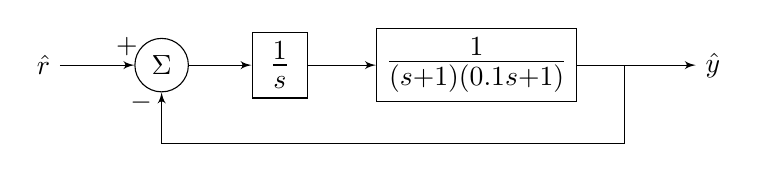
\begin{tikzpicture}[node distance=1.5cm,auto,>=latex']
	\node [input] (r) {$\hat{r}$};
	\node [sum] (sumr) [right of=r] {$\Sigma$};
	\node [block] (gc) [right of=sumr] {\Large$ \frac{1}{s} $};
	\node [block] (gp) [right of=gc,node distance=2.5cm] {\Large$ \frac{1}{(s+1)(0.1s+1)} $};
	\node [output] (y) [right of=gp,node distance=3cm]{$\hat{y}$};
	\node [waypoint] (wp) [below of=gp,node distance=1cm] {};
	
	\draw[->] (r) -- node[pos=0.9] {$+$} (sumr);
	\draw[->] (sumr) -- (gc);
	\draw[->] (gc) --  (gp);
	\draw[->] (gp) -- (y);
	\draw[->] ($ (gp)!0.625!(y) $) |- (wp)-| node[pos=0.9] {$-$} (sumr);
	\end{tikzpicture}
\end{center}
\[ L=G_cG_p = \frac{1}{s(s+1)(0.1s+1)} \]
Use superposition to sketch Bode plots.
\begin{center}
	\begin{minipage}{0.49\textwidth}
		\centering
		Asymptote Plot\\
		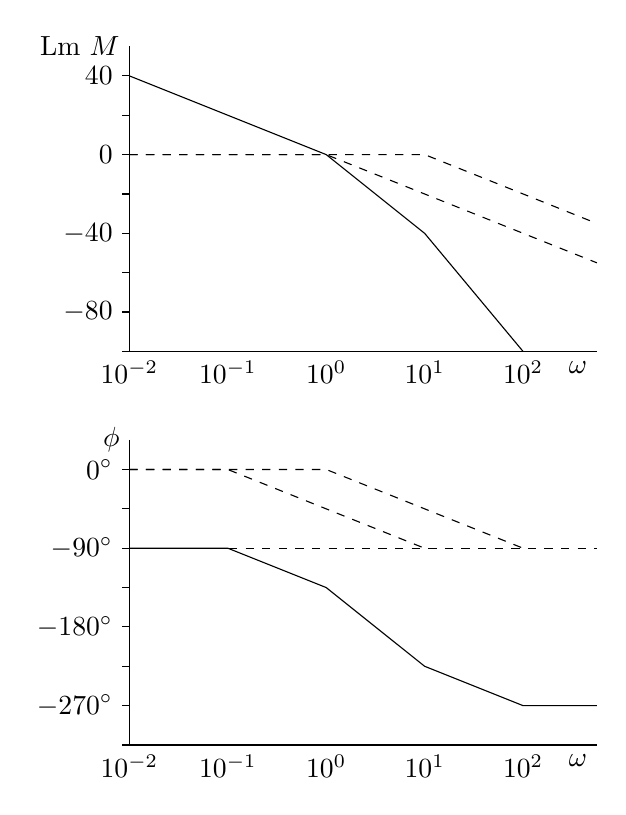
\begin{tikzpicture}[xscale=1.25,yscale=0.025]
		% magnitude plot
		\draw (-2,55) node[left] {$\Lm M$} |- (2.75,-100) node[below left] {$ \omega $};
		
		\foreach \x in {-2,-1,0,1,2} \draw[yshift=-100cm] (\x cm,0pt) -- (\x cm,-2pt) node[anchor=north] {$10^{\x}$};
		
		\foreach \y in {20,-20,-60,-100} \draw[xshift=-2cm] (0pt,\y cm) -- (-2pt,\y cm) node[anchor=east] {};
		\foreach \y in {40,0,-40,-80} \draw[xshift=-2cm] (0pt,\y cm) -- (-2pt,\y cm) node[anchor=east] {$\y$};
		 
		\draw (-2,40) -- (0,0) -- (1,-40) -- (2,-100);
		\draw[dashed] (-2,0) -- (0,0) -- (2.75,-55);
		\draw[dashed] (-2,0) -- (1,0) -- (2.75,-35);
		
		
		% phase plot
		\draw[yshift=-200cm] (-2,55) node[left] {$\phi$} |- (2.75,-100) node[below left] {$ \omega $};
		
		\foreach \x in {-2,-1,0,1,2} \draw[yshift=-300cm] (\x cm,0pt) -- (\x cm,-2pt) node[anchor=north] {$10^{\x}$};
		
		\foreach \y [evaluate=\y as \yeval using (\y*4/9)+40] in {0,-90,-180,-270} \draw[xshift=-2cm,yshift=-200cm] (0pt,\yeval cm) -- (-2pt,\yeval cm) node[anchor=east] {$\y^\circ$};
		\foreach \y [evaluate=\y as \yeval using (\y*4/9)+40] in {-45,-135,-225,-315} \draw[xshift=-2cm,yshift=-200cm] (0pt,\yeval cm) -- (-2pt,\yeval cm) node[anchor=east] {};
		
		\draw[dashed,yshift=-200cm] (-2,-0) -- (2.75,0);
		\draw[dashed,yshift=-200cm] (-2,40) -- (-1,40) -- (1,0);
		\draw[dashed,yshift=-200cm] (-2,40) -- (0,40) -- (2,0);
		\draw[yshift=-200cm] (-2,0) -- (-1,0) -- (0,-20) -- (1,-60) -- (2,-80) -- (2.75,-80);
			
		\end{tikzpicture}
	\end{minipage}
	\begin{minipage}{0.49\textwidth}
		\centering
		Actual Plot\\
		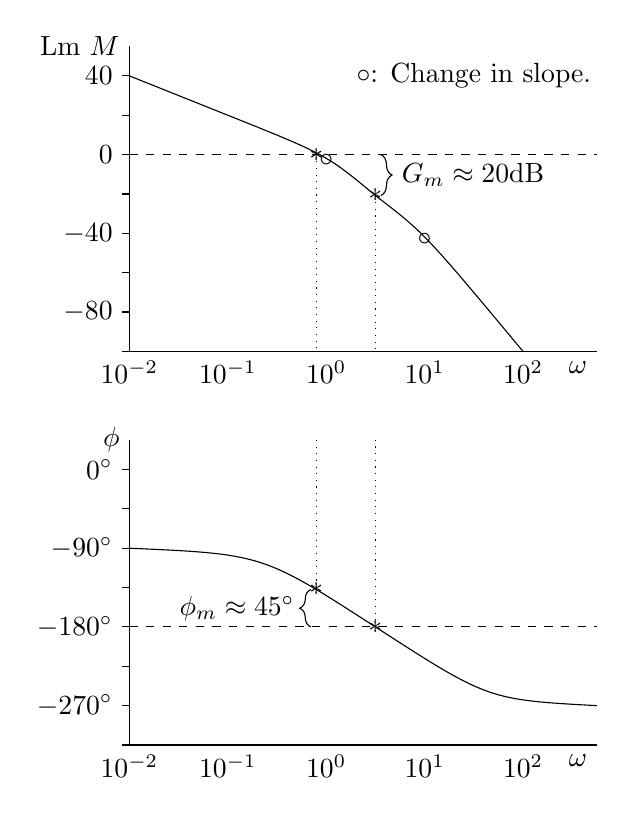
\begin{tikzpicture}[xscale=1.25,yscale=0.025]
		% magnitude plot
		\draw (-2,55) node[left] {$\Lm M$} |- (2.75,-100) node[below left] {$ \omega $};
		
		\foreach \x in {-2,-1,0,1,2} \draw[yshift=-100cm] (\x cm,0pt) -- (\x cm,-2pt) node[anchor=north] {$10^{\x}$};
		
		\foreach \y in {20,-20,-60,-100} \draw[xshift=-2cm] (0pt,\y cm) -- (-2pt,\y cm) node[anchor=east] {};
		\foreach \y in {40,0,-40,-80} \draw[xshift=-2cm] (0pt,\y cm) -- (-2pt,\y cm) node[anchor=east] {$\y$};
		
		\draw[dashed] (-2,0) -- (2.75,0); 
		\draw (-2,40) -- (-1,20) ..controls (0,0) .. (0.5,-20.8) ..controls (1,-40) .. (2,-100);
		
		\draw[dotted] (-0.1,0) node {$ * $} -- (-0.1,-100);
		\draw[dotted] (0.5,-20.8) node {$ * $} -- (0.5,-100);
		
		\draw [decorate,decoration={brace,amplitude=4pt}, xshift=1.6pt,yshift=0pt] (0.5,0) -- (0.5,-20.8) node [right,black,midway,xshift=4pt] {$G_m\approx20$dB};
		
		\node at (0,-3) {$ \circ $};
		\node at (1,-43) {$ \circ $};
		\node[align=left] at (1.5,40) {$ \circ $: Change in slope.};
		
		% phase plot
		\draw[yshift=-200cm] (-2,55) node[left] {$\phi$} |- (2.75,-100) node[below left] {$ \omega $};
		
		\foreach \x in {-2,-1,0,1,2} \draw[yshift=-300cm] (\x cm,0pt) -- (\x cm,-2pt) node[anchor=north] {$10^{\x}$};
		
		\foreach \y [evaluate=\y as \yeval using (\y*4/9)+40] in {0,-90,-180,-270} \draw[xshift=-2cm,yshift=-200cm] (0pt,\yeval cm) -- (-2pt,\yeval cm) node[anchor=east] {$\y^\circ$};
		\foreach \y [evaluate=\y as \yeval using (\y*4/9)+40] in {-45,-135,-225,-315} \draw[xshift=-2cm,yshift=-200cm] (0pt,\yeval cm) -- (-2pt,\yeval cm) node[anchor=east] {};
		
		\draw[dashed,yshift=-200cm] (-2,-40) -- (2.75,-40);
		\draw[yshift=-200cm] (-2,0) ..controls (-0.6453,-3) .. (0.5,-40) ..controls (1.6453,-77) .. (2.75,-80);
		
		\draw[dotted,yshift=-200cm] (-0.1,55) -- (-0.1,-21) node {$ * $};
		\draw[dotted,yshift=-200cm] (0.5,-40) node {$ * $} -- (0.5,55);
		
		\draw [decorate,decoration={brace,amplitude=4pt}, xshift=-1.6pt,yshift=-200cm] (-0.1,-40) -- (-0.1,-21) node [left,black,midway,xshift=-2.4pt] {$\phi_m\approx 45^\circ$};		
		\end{tikzpicture}
	\end{minipage}
\end{center}
Both the gain and phase margin ar greater than zero, so the system is stable.
\clearpage
\exmp
Find the gain and phase margin for the following system.
\begin{center}
	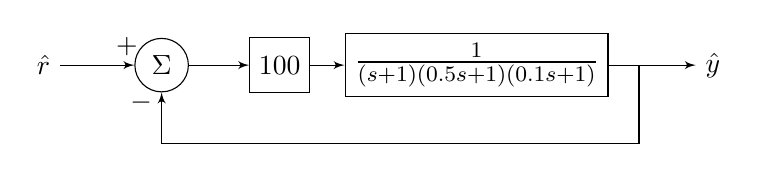
\begin{tikzpicture}[node distance=1.5cm,auto,>=latex']
	\node [input] (r) {$\hat{r}$};
	\node [sum] (sumr) [right of=r] {$\Sigma$};
	\node [block] (gc) [right of=sumr] {$ 100 $};
	\node [block] (gp) [right of=gc,node distance=2.5cm] {\large$ \frac{1}{(s+1)(0.5s+1)(0.1s+1)} $};
	\node [output] (y) [right of=gp,node distance=3cm]{$\hat{y}$};
	\node [waypoint] (wp) [below of=gp,node distance=1cm] {};
	
	\draw[->] (r) -- node[pos=0.9] {$+$} (sumr);
	\draw[->] (sumr) -- (gc);
	\draw[->] (gc) --  (gp);
	\draw[->] (gp) -- (y);
	\draw[->] ($ (gp)!0.6875!(y) $) |- (wp)-| node[pos=0.9] {$-$} (sumr);
	\end{tikzpicture}
\end{center}
\[ L=G_cG_p = \frac{100}{(s+1)(0.5s+1)(0.1s+1)} \]
Use superposition to sketch Bode plots.
\begin{center}
	\begin{minipage}{0.49\textwidth}
		\centering
		Asymptote Plot\\
		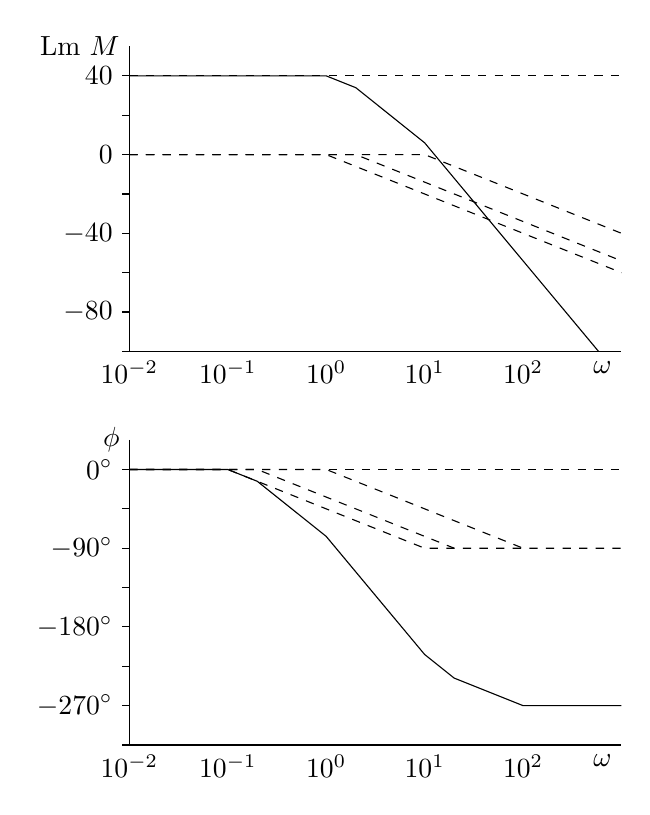
\begin{tikzpicture}[xscale=1.25,yscale=0.025]
		% magnitude plot
		\draw (-2,55) node[left] {$\Lm M$} |- (3,-100) node[below left] {$ \omega $};
		
		\foreach \x in {-2,-1,0,1,2} \draw[yshift=-100cm] (\x cm,0pt) -- (\x cm,-2pt) node[anchor=north] {$10^{\x}$};
		
		\foreach \y in {20,-20,-60,-100} \draw[xshift=-2cm] (0pt,\y cm) -- (-2pt,\y cm) node[anchor=east] {};
		\foreach \y in {40,0,-40,-80} \draw[xshift=-2cm] (0pt,\y cm) -- (-2pt,\y cm) node[anchor=east] {$\y$};
		 		
		\draw (-2,40) -- (0,40) -- (0.301,34) -- (1,6) -- (2.767,-100);
		\draw[dashed] (-2,40) -- (3,40);
		\draw[dashed] (-2,0) -- (0,0) -- (3,-60);
		\draw[dashed] (-2,0) -- (.301,0) -- (3,-54);
		\draw[dashed] (-2,0) -- (1,0) -- (3,-40);
		
		% phase plot
		\draw[yshift=-200cm] (-2,55) node[left] {$\phi$} |- (3,-100) node[below left] {$ \omega $};
		
		\foreach \x in {-2,-1,0,1,2} \draw[yshift=-300cm] (\x cm,0pt) -- (\x cm,-2pt) node[anchor=north] {$10^{\x}$};
		
		\foreach \y [evaluate=\y as \yeval using (\y*4/9)+40] in {0,-90,-180,-270} \draw[xshift=-2cm,yshift=-200cm] (0pt,\yeval cm) -- (-2pt,\yeval cm) node[anchor=east] {$\y^\circ$};
		\foreach \y [evaluate=\y as \yeval using (\y*4/9)+40] in {-45,-135,-225,-315} \draw[xshift=-2cm,yshift=-200cm] (0pt,\yeval cm) -- (-2pt,\yeval cm) node[anchor=east] {};
		
		\draw[dashed,yshift=-200cm] (-2,40) -- (3,40);
		\draw[dashed,yshift=-200cm] (-2,40) -- (-1,40) -- (1,0) -- (3,0);
		\draw[dashed,yshift=-200cm] (-2,40) -- (-0.7,40) -- (1.3,0);
		\draw[dashed,yshift=-200cm] (-2,40) -- (0,40) -- (2,0);
		\draw[yshift=-200cm] (-2,40) -- (-1,40) -- (-0.7,34) -- (0,6) -- (1,-54) -- (1.3,-66) -- (2,-80) -- (3,-80);
		
		\end{tikzpicture}
	\end{minipage}
\begin{minipage}{0.49\textwidth}
	\centering
	Actual Plot\\
		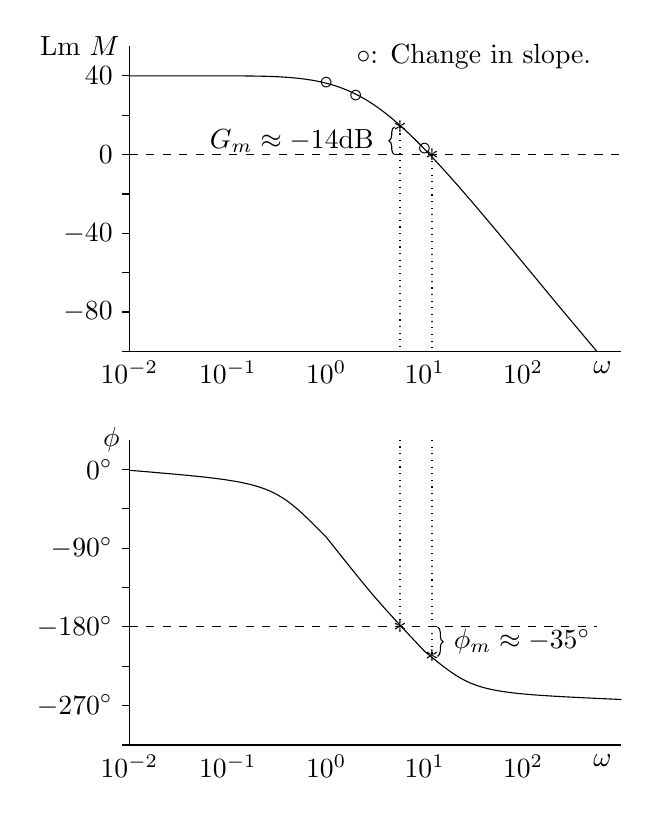
\begin{tikzpicture}[xscale=1.25,yscale=0.025]
		% magnitude plot
		\draw (-2,55) node[left] {$\Lm M$} |- (3,-100) node[below left] {$ \omega $};
		
		\foreach \x in {-2,-1,0,1,2} \draw[yshift=-100cm] (\x cm,0pt) -- (\x cm,-2pt) node[anchor=north] {$10^{\x}$};
		
		\foreach \y in {20,-20,-60,-100} \draw[xshift=-2cm] (0pt,\y cm) -- (-2pt,\y cm) node[anchor=east] {};
		\foreach \y in {40,0,-40,-80} \draw[xshift=-2cm] (0pt,\y cm) -- (-2pt,\y cm) node[anchor=east] {$\y$};
		
		\draw[dashed] (-2,0) -- (3,0); 
		\draw (-2,40) -- (-1.125,40) ..controls (0.434,40) .. (2.345,-75.88) -- (2.75,-100);
		
		\draw[dotted] (1.075,0) node {$ * $} -- (1.075,-100);
		
		\draw[dotted] (0.75,14.1) node {$ * $} -- (0.75,-100);
		\draw [decorate,decoration={brace,amplitude=2pt}, xshift=-1.6pt,yshift=0pt] (0.75,0) -- (0.75,14.1) node [left,black,midway,xshift=-4pt] {$G_m\approx-14$dB};
		
		\node at (0,36) {$ \circ $};
		\node at (.301,29.8) {$ \circ $};
		\node at (1,2.8) {$ \circ $};
		\node[align=left] at (1.5,50) {$ \circ $: Change in slope.};
		
		
		% phase plot
		\draw[yshift=-200cm] (-2,55) node[left] {$\phi$} |- (3,-100) node[below left] {$ \omega $};
		
		\foreach \x in {-2,-1,0,1,2} \draw[yshift=-300cm] (\x cm,0pt) -- (\x cm,-2pt) node[anchor=north] {$10^{\x}$};
		
		\foreach \y [evaluate=\y as \yeval using (\y*4/9)+40] in {0,-90,-180,-270} \draw[xshift=-2cm,yshift=-200cm] (0pt,\yeval cm) -- (-2pt,\yeval cm) node[anchor=east] {$\y^\circ$};
		\foreach \y [evaluate=\y as \yeval using (\y*4/9)+40] in {-45,-135,-225,-315} \draw[xshift=-2cm,yshift=-200cm] (0pt,\yeval cm) -- (-2pt,\yeval cm) node[anchor=east] {};
		
		\draw[dashed,yshift=-200cm] (-2,-40) -- (2.75,-40);
		\draw[yshift=-200cm] (-2,39.6) ..controls (-0.5487,33.5) .. (0,5.644) ..controls (0.5,-25.78).. (1,-52.44) ..controls (1.5143,-73.5) .. (3,-76.88);
		
		\draw[dotted,yshift=-200cm] (0.75,-40) node {$ * $} -- (0.75,55);
		
		\draw[dotted,yshift=-200cm] (1.075,55) -- (1.075,-55) node {$ * $};
		\draw [decorate,decoration={brace,amplitude=2pt}, xshift=1.6pt,yshift=-200cm] (1.075,-40) -- (1.075,-55) node [right,black,midway,xshift=2.4pt] {$\phi_m\approx-35^\circ$};		
		\end{tikzpicture}
\end{minipage}
\end{center}
Both the gain and phase margin ar less than zero, so the system is \textbf{unstable}.
\clearpage
\exmp
Find the gain and phase margin for the following system.
\begin{center}
	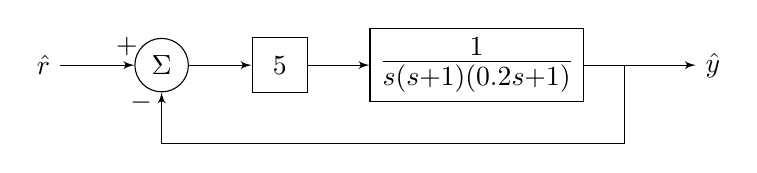
\begin{tikzpicture}[node distance=1.5cm,auto,>=latex']
	\node [input] (r) {$\hat{r}$};
	\node [sum] (sumr) [right of=r] {$\Sigma$};
	\node [block] (gc) [right of=sumr] {$ 5 $};
	\node [block] (gp) [right of=gc,node distance=2.5cm] {\Large$ \frac{1}{s(s+1)(0.2s+1)} $};
	\node [output] (y) [right of=gp,node distance=3cm]{$\hat{y}$};
	\node [waypoint] (wp) [below of=gp,node distance=1cm] {};
	
	\draw[->] (r) -- node[pos=0.9] {$+$} (sumr);
	\draw[->] (sumr) -- (gc);
	\draw[->] (gc) --  (gp);
	\draw[->] (gp) -- (y);
	\draw[->] ($ (gp)!0.625!(y) $) |- (wp)-| node[pos=0.9] {$-$} (sumr);
	\end{tikzpicture}
\end{center}
\[ L=G_cG_p = \frac{1}{s(s+1)(0.2s+1)} \]
Use superposition to sketch Bode plots.
\begin{center}
	\begin{minipage}{0.49\textwidth}
		\centering
		Asymptote Plot\\
		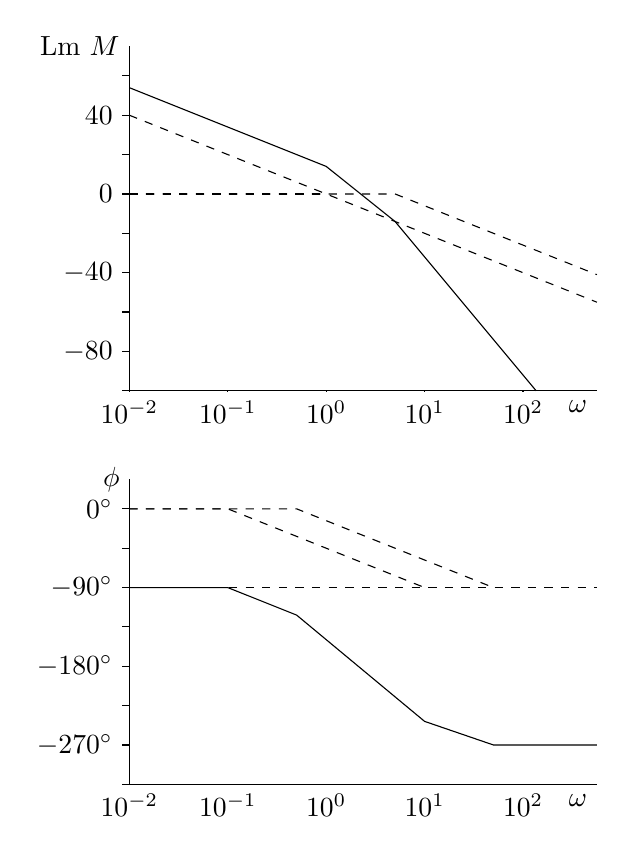
\begin{tikzpicture}[xscale=1.25,yscale=0.025]
		% magnitude plot
		\draw (-2,75) node[left] {$\Lm M$} |- (2.75,-100) node[below left] {$ \omega $};
		
		\foreach \x in {-2,-1,0,1,2} \draw[yshift=-100cm] (\x cm,0pt) -- (\x cm,-2pt) node[anchor=north] {$10^{\x}$};
		
		\foreach \y in {60,20,-20,-60,-100} \draw[xshift=-2cm] (0pt,\y cm) -- (-2pt,\y cm) node[anchor=east] {};
		\foreach \y in {40,0,-40,-80} \draw[xshift=-2cm] (0pt,\y cm) -- (-2pt,\y cm) node[anchor=east] {$\y$};
		
		\draw[dashed] (-2,40) -- (2.75,-55);
		\draw[dashed] (-2,0) -- (0,0);
		\draw[dashed] (-2,0) -- (0.7,0) -- (2.75,-41);
		\draw (-2,54) -- (0,14) -- (0.7,-14) -- (2.133,-100);

		
		% phase plot
		\draw[yshift=-200cm] (-2,55) node[left] {$\phi$} |- (2.75,-100) node[below left] {$ \omega $};
		
		\foreach \x in {-2,-1,0,1,2} \draw[yshift=-300cm] (\x cm,0pt) -- (\x cm,-2pt) node[anchor=north] {$10^{\x}$};
		
		\foreach \y [evaluate=\y as \yeval using (\y*4/9)+40] in {0,-90,-180,-270} \draw[xshift=-2cm,yshift=-200cm] (0pt,\yeval cm) -- (-2pt,\yeval cm) node[anchor=east] {$\y^\circ$};
		\foreach \y [evaluate=\y as \yeval using (\y*4/9)+40] in {-45,-135,-225,-315} \draw[xshift=-2cm,yshift=-200cm] (0pt,\yeval cm) -- (-2pt,\yeval cm) node[anchor=east] {};
		
		\draw[dashed,yshift=-200cm] (-2,-0) -- (2.75,0);
		\draw[dashed,yshift=-200cm] (-2,40) -- (-1,40) -- (1,0);
		\draw[dashed,yshift=-200cm] (-2,40) -- (-0.3,40) -- (1.7,0);
		\draw[yshift=-200cm] (-2,0) -- (-1,0) -- (-0.3,-14) -- (1,-68) -- (1.7,-80) -- (2.75,-80);
		
			
		\end{tikzpicture}
	\end{minipage}
\begin{minipage}{0.49\textwidth}
	\centering
	Actual Plot\\
		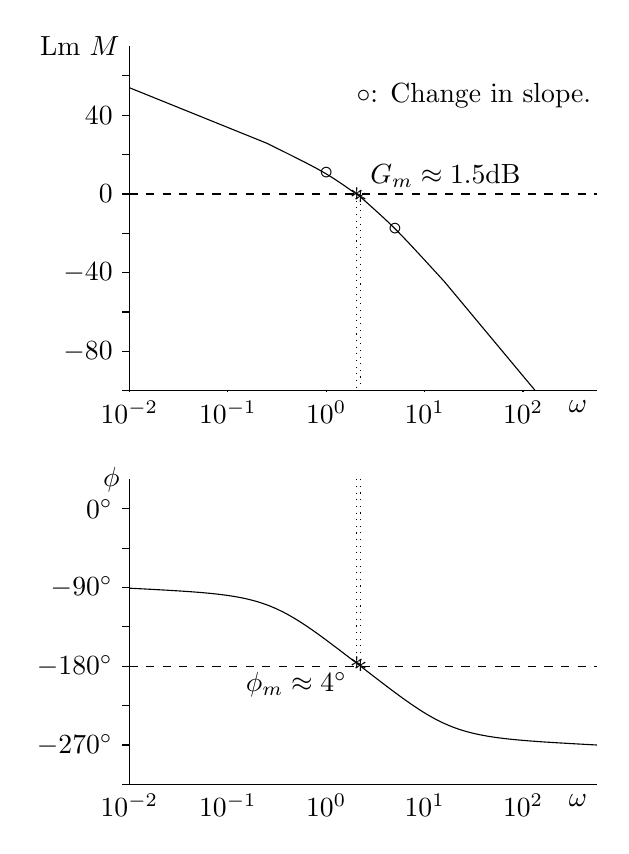
\begin{tikzpicture}[xscale=1.25,yscale=0.025]
		% magnitude plot
		\draw (-2,75) node[left] {$\Lm M$} |- (2.75,-100) node[below left] {$ \omega $};
		
		\foreach \x in {-2,-1,0,1,2} \draw[yshift=-100cm] (\x cm,0pt) -- (\x cm,-2pt) node[anchor=north] {$10^{\x}$};
		
		\foreach \y in {60,20,-20,-60,-100} \draw[xshift=-2cm] (0pt,\y cm) -- (-2pt,\y cm) node[anchor=east] {};
		\foreach \y in {40,0,-40,-80} \draw[xshift=-2cm] (0pt,\y cm) -- (-2pt,\y cm) node[anchor=east] {$\y$};
		
		\draw[dashed] (-2,0) -- (2.75,0); 
		\draw (-2,54) -- (-0.6,25.7) ..controls (0,10.8) .. (0.35,-1.6) ..controls (0.7,-17.2) .. (1.2,-44.5) -- (2.125,-100);
		
		\draw[dotted] (0.31,0) node {$ * $} -- (0.31,-100);
		\draw[dotted] (0.35,-1.6) node {$ * $} node[above right] {$ G_m \approx 1.5 $dB} -- (0.35,-100);
		
		\node at (0,10.5) {$ \circ $};
		\node at (.699,-18) {$ \circ $};
		\node[align=left] at (1.5,50) {$ \circ $: Change in slope.};
		
		% phase plot
		\draw[yshift=-200cm] (-2,55) node[left] {$\phi$} |- (2.75,-100) node[below left] {$ \omega $};
		
		\foreach \x in {-2,-1,0,1,2} \draw[yshift=-300cm] (\x cm,0pt) -- (\x cm,-2pt) node[anchor=north] {$10^{\x}$};
		
		\foreach \y [evaluate=\y as \yeval using (\y*4/9)+40] in {0,-90,-180,-270} \draw[xshift=-2cm,yshift=-200cm] (0pt,\yeval cm) -- (-2pt,\yeval cm) node[anchor=east] {$\y^\circ$};
		\foreach \y [evaluate=\y as \yeval using (\y*4/9)+40] in {-45,-135,-225,-315} \draw[xshift=-2cm,yshift=-200cm] (0pt,\yeval cm) -- (-2pt,\yeval cm) node[anchor=east] {};
		
		\draw[dashed,yshift=-200cm] (-2,-40) -- (2.75,-40);
		\draw[yshift=-200cm] (-2,-0.311) ..controls (-0.5850,-4) .. (0.35,-40) ..controls (1.2822,-76) .. (2.75,-80);
		
		\draw[dotted,yshift=-200cm] (0.35,-40) node {$ * $} -- (0.35,55);	
		\draw[dotted,yshift=-200cm] (0.31,55) -- (0.31,-38.2) node {$ * $} node[below left] {$ \phi_m\approx4^\circ $};			
		\end{tikzpicture}
\end{minipage}
\end{center}
Both the gain and phase margin ar greater than zero, so the system is stable. However, it is \textbf{not robust}, because the gain and phase margins are too small. This would be a risky design.

\section*{Determining the Phase from the Gain Margins}
\begin{itemize}
	\item If $ G_cG_p $ has no zeros or poles in the RHP, we call it a stable minimum phase system. In this case, if $ G_m>0 $ then $ P_m $ is also $ >0 $ --- there will never be a case where one is $ >0 $ while the other is $ <0 $.
	\item This means that  we can use only the gain plot to determine stability by using the following procedure:
	\item Since every pole adds $ -20 $dB/decade to slope of $ \Lm $ and $ -90^\circ $ to $ \phi $, we can estimate the phase at the crossover frequency by looking at the slope as the Lm crosses 0dB.
	\begin{center}
		\begin{tabular}{c|c|c}
			\begin{minipage}{0.16\textwidth}
				\centering
				Slope of $ \Lm $ asymptote at 0dB crossover
				\vspace{2pt}
			\end{minipage} & 
			\begin{minipage}{0.16\textwidth}
				\centering
				Approximate phase
				\vspace{2pt}
			\end{minipage} &
			\begin{minipage}{0.16\textwidth}
				\centering
				Phase margin $ \phi_m $
				\vspace{2pt}
			\end{minipage}\\ \hline\vspace{2pt}
			$ -20 $dB/decade & $ -90^\circ $ & $ 90^\circ $ (Stable) \\\vspace{2pt}
			$ -40 $dB/decade & $ -180^\circ $ & $ 0^\circ $ (Marginal)\\\vspace{2pt}
			$ -60 $dB/decade & $ -270^\circ $ & $ -90^\circ $ (Unstable)
		\end{tabular}
	\end{center}
	\item This tells us that we want the slope of the asymptote of $ \Lm G_c G_p $ to be $ -20 $dB/decade at or near the crossover.
	\begin{center}
		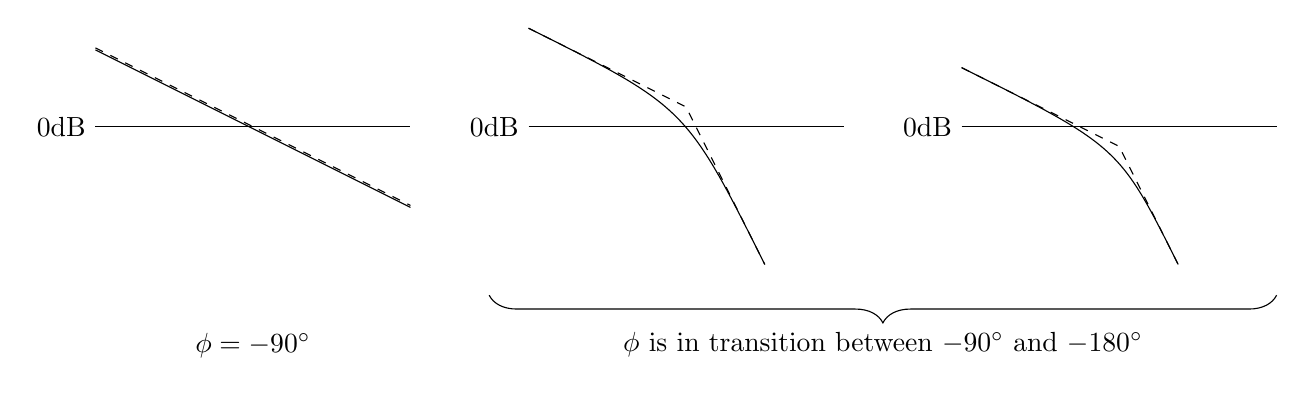
\begin{tikzpicture}
		\draw (0,0) node[left] {0dB} -- (4,0);
		\draw[xshift=5.5cm] (0,0) node[left] {0dB} -- (4,0);
		\draw[xshift=11cm] (0,0) node[left] {0dB} -- (4,0);
		
		\draw[dashed] (0,1) -- (4,-1);
		\draw (0,0.975) -- (4,-1.025);
		\node[below,align=center] at (2,-2.5) {$ \phi=-90^\circ $};
		
		\draw[dashed,xshift=5.5cm] (0,1.25) -- (2,0.25) -- (3,-1.75);
		\draw[xshift=5.5cm] (0,1.25) ..controls (2,0.25) .. (3,-1.75);
		
		\draw[dashed,xshift=11cm] (0,0.75) -- (2,-0.25) -- (2.75,-1.75);
		\draw[xshift=11cm] (0,0.75) ..controls (2,-0.25) .. (2.75,-1.75);
		
		\draw [decorate,decoration={brace,amplitude=10pt}, yshift=-4pt] (15,-2) -- (5,-2) node [below,black,midway,yshift=-10pt,align=center] {$ \phi $ is in transition between $ -90^\circ $ and $ -180^\circ $};
		\end{tikzpicture}
	\end{center}
	\item Now we know how to achieve our primary goals (disturbance rejection, noise attenuation, stability robustness):
	\begin{itemize}
		\item $ \Lm G_cG_p $ is large for small $ \omega $ (disturbance rejection)
		\item $ \Lm G_cG_p $ is small for large $ \omega $ (noise attenuation)
		\item \textbf{The slope of $ \Lm G_cG_p $ is $ -20 $dB/decade at or near the 0dB crossover (robust stability)}
	\end{itemize}
	\item Now let's look at how to meet our secondary goals.
\end{itemize}

\section*{Time Response Considerations}
\subsection*{Steady-State Error}
\begin{itemize}
	\item If $ \Lm G_cG_p $ is large at small $ \omega $, $ e_{ss} $ will be small.
	\item Justification: for $ \Lm G_cG_p $ to be large at small $ \omega $, $ G_cG_p $ must have a pole at/near 0 or a very high gain. %We saw in the root locus controller design that both of these reduce $ e_{ss} $.
	\item So, we have already taken care of $ e_{ss} $ when we made $ \Lm G_cG_p $ large at small $ \omega $ for disturbance rejection.
	\[ T=\frac{G_cG_p}{1+G_cG_p} \quad\Rightarrow\quad G_cG_p \gg 1 \text{ at low fre.} \quad\Rightarrow\quad T=1 \quad\Rightarrow\quad Y = R \]
\end{itemize}
\subsection*{Transient Behavior:}
\begin{center}
	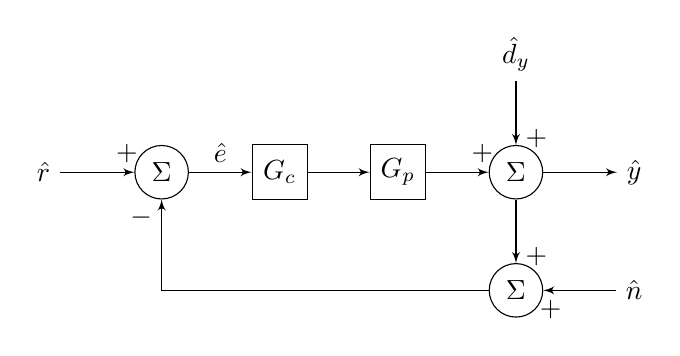
\begin{tikzpicture}[node distance=1.50cm,auto,>=latex']
	\node [input] (r) {$\hat{r}$};
	\node [sum] (sumr) [right of=r] {$\Sigma$};
	\node [block] (gc) [right of=sumr] {$ G_c $};
	\node [block] (gp) [right of=gc] {$ G_p $};
	\node [sum] (sumy) [right of=gp] {$\Sigma$};
	\node [output] (y) [right of=sumy]{$\hat{y}$};
	\node [sum] (sumn) [below of=sumy] {$\Sigma$};
	\node [input] (n) [right of=sumn,align=center]{$ \hat{n} $};
	\node [input] (dy) [above of=sumy,node distance=1.5cm]{$ \hat{d}_y $};
	
	\draw[->] (r) -- node[pos=0.9] {$+$} (sumr);
	\draw[->] (sumr) -- node {$\hat{e}$} (gc);
	\draw[->] (gc) -- (gp);
	\draw[->] (gp) -- node[pos=0.9] {$+$} (sumy);		
	\draw[->] (dy) -- node[pos=0.9] {$+$} (sumy);
	\draw[->] (sumy) -- (y);
	\draw[->] (sumy) -- node[pos=0.9] {$+$} (sumn);
	\draw[->] (n) -- node[pos=0.9] {$+$} (sumn);
	\draw[->] (sumn) -| node[pos=0.9] {$-$} (sumr);
	\end{tikzpicture}
\end{center}
\begin{itemize}
	\item Transient behavior of the system is governed by
	\[ \frac{\hat{y}}{\hat{r}} = \frac{G_cG_p}{1+G_cG_p} = T \]
	\item If we want to set $ t_{rise} $, $ t_{settle} $, $ t_{peak} $, $ \%OS $, etc... then CLTF must be similar to a 2nd order system.%As in root-locus design, 
	\[ T \approx \frac{\omega_n^2}{s^2+2\zeta\omega_ns + \omega_n^2} \]
	where $ \zeta $ and $ \omega_n $ are chosen based on designed transient performance.
	\item What does that mean for $ G_cG_p $?
	\begin{itemize}
		\item Find an expression of $ G_cG_p $ in terms of $ T $
	\end{itemize}
	\[ T = \frac{G_cG_p}{1+G_cG_p} \quad\rightarrow\quad T(1+G_cG_p) = G_cG_p \]
	\[ T = G_cG_p - G_cG_p (T) \]
	\[ \boxed{G_cG_p = \frac{T}{1-T}} \]
	\begin{itemize}
		\item Find expression for $ G_cG_p $ in terms of $ \zeta $ and $ \omega_n $
	\end{itemize}
	\begin{align*}
	G_cG_p &= \frac{\frac{\omega_n^2}{s^2+2\zeta\omega_ns + \omega_n^2}}{1-\frac{\omega_n^2}{s^2+2\zeta\omega_ns + \omega_n^2}} = \frac{\omega_n^2}{s^2+2\zeta\omega_ns + \omega_n^2 - \omega_n^2}\\
	& = \frac{\omega_n^2}{s^2+2\omega_n\zeta s} = \frac{\omega_n^2}{s(s+2\omega_n\zeta)}\\
	\end{align*}
	\[ \boxed{G_cG_p = \frac{\frac{\omega_n}{2\zeta}}{s\left(\frac{s}{2\zeta\omega_n}+1\right)}} \]
	\item The Bode diagram of $ G_cG_p $ will look like:
		\begin{center}
			\begin{tikzpicture}[xscale=1.25]
			\draw (0,3.5) node[left] {$\Lm M$} |- (4,0) node[below left] {$ \omega $};
			\draw (0,3.25) -- (0.5,3) ..controls (2,2.25) .. (2.5,1.25) -- (3.125,0);
			\draw[dashed] (2,2.125) -- (2,0);
			\draw[->] (2.5,2.5) node[right] {Corner at $ 2\zeta\omega_n $} -- (2,2.125);
			
			\draw[yshift=-4.5cm] (0,3.5) node[left] {$\phi$} |- (4,0) node[below left] {$ \omega $};
			\draw[yshift=-4.5cm] (0,2.75) -- (1,2.75) ..controls (1.5,2.75) and (1.75,2.75) .. (2,1.75) ..controls (2.25,.75) and (2.5,.75) .. (3,.75) -- (4,.75);
			\draw[dashed,yshift=-4.5cm] (0,2.75) node[left]{$- 90^\circ $} -- (2.5,2.75);
			\draw[dashed,yshift=-4.5cm] (1.5,0.75) -- (4,0.75);
			\node[left,yshift=-4.5cm] at (0,0.75) {$- 180^\circ $};
			\end{tikzpicture}
		\end{center}
	\item Where is the 0dB line? Let's use the low-frequency asymptote to estimate it.
	\[ G_cG_p(\jw) = \frac{\omega_n}{2\zeta(\jw)\left(\frac{\jw}{2\zeta\omega_n}+1\right)} \]
	\[ \left|G_cG_p(\jw)\right| = \frac{\omega_n}{2\zeta\omega\sqrt{\frac{\omega^2}{4\zeta^2\omega_n^2}+1}} \]
	Approximate $ \left|G_cG_p(\jw)\right| $ when $ \omega $ is small ($ \omega \ll \omega_n $)
	\[ \left|G_cG_p(\jw)\right| \approx \frac{\omega_n}{2\zeta\omega} \]
	\item Our low-frequency asymptote will have slope of $ -20 $dB/decade and intercept 0dB when
	\[ \frac{\omega_n}{2\zeta\omega} = 1 \quad\Rightarrow\quad \omega = \frac{\omega_n}{2\zeta} \]
	\item To meet transient requirements $ \Lm|G_cG_p| $ must have:
	\begin{itemize}
		\item A low-$ \omega $ asymptote with $ -20 $dB/decade slope and a 0dB intercept at $ \omega=\omega_n/2\zeta $.
		\item A ``corner'' decreasing the slope to $ -40 $dB/decade at $ \omega=2\zeta\omega_n $.
	\end{itemize}
	\item Note that if $ \zeta < \frac{1}{2} $ the corner will be before the low-$ \omega $ asymptote gets to 0dB.
	\begin{center}
		\begin{tikzpicture}
			\draw (0,0) node[left] {0dB} -- (4,0);
			\draw (0,0.5) -- (2,-0.5) -- ( 3,-1.5);
			\draw [decorate,decoration={brace,amplitude=10pt}, yshift=-4pt] (4.25,-2) -- (-0.75,-2) node [below,black,midway,yshift=-10pt,align=center] {$ \zeta>\frac{1}{2} $};
			\node[below] at (1,0) {$ \frac{\omega_n}{2\zeta} $};
			\draw[dashed] (2,0) node[above] {$ 2\zeta\omega_n $} -- (2,-0.5);
			\node at (1,0) {$ * $};
			
			\draw[xshift=5.5cm] (0,0) node[left] {0dB} -- (4,0);
			\draw[xshift=5.5cm] (0,1) -- (2,0) -- (3.5,-1.5);
			\draw [decorate,decoration={brace,amplitude=10pt}, yshift=-4pt] (9.75,-2) -- (4.75,-2) node [below,black,midway,yshift=-10pt,align=center] {$ \zeta=\frac{1}{2} $};
			\node[above right] at (7.5,0) {$ 2\zeta\omega_n = \frac{\omega_n}{2\zeta} $};
			\node at (7.5,0) {$ * $};
			
			\draw[xshift=11cm] (0,0) node[left] {0dB} -- (4,0);
			\draw[xshift=11cm] (0,1.5) -- (2,0.5) -- (3.75,-1.5);
			\draw [decorate,decoration={brace,amplitude=10pt}, yshift=-4pt] (15.25,-2) -- (10.25,-2) node [below,black,midway,yshift=-10pt,align=center] {$ \zeta<\frac{1}{2} $};\node[below] at (1,0) {$ \frac{\omega_n}{2\zeta} $};
			\draw[dashed] (13,0.5) -- (13,0) node[below] {$ 2\zeta\omega_n $};
			\node[above right] at (13.5,0) {$ \frac{\omega_n}{2\zeta} $};
			\node at (13.5,0) {$ * $};
		\end{tikzpicture}
	\end{center}
\end{itemize}

\end{document}